\documentclass[../main.tex]{subfiles}

\begin{document}
%%%%%%%%%%%%%%%%%%%%%%%%%%%%%%%%%%%%%%%%%%%%%%%%%%%%%%%
%   New Chapter                                       %
%%%%%%%%%%%%%%%%%%%%%%%%%%%%%%%%%%%%%%%%%%%%%%%%%%%%%%%

\chapter{Data Clustering and Mixture Models}

%\begin{chapquote}{Author's name, \textit{Source of this quote}}
%``This is a quote and I don't know who said this.''
%\end{chapquote}
In section \ref{sec_4_EM}, we discussed K-means and (Gaussian) mixture models in order to motivate the EM algorithm, while in this chapter we revisit these methods from a view of data clustering. Most of the basic ideas have already been covered in section \ref{sec_4_EM}, and we recommend readers who are interested in more detailed analysis to go through section \ref{sec_4_EM}. Despite the overlapping of the content, in this chapter we will see some recent extensions for K-means to give better guarantees of the performance and handle large data set. We will also briefly discuss about classical model selection methods.
\section{Motivation}
In previous chapters, we have discussed various methods of data reduction, such as PCA and linear autoencoders. Data clustering, however, provide us a different way to look at the reduction problem. Think about a user analysis problem, where we have data of thousands of users and want to extract some useful information. A natural idea is to group similar users together and represent these users with some representative properties, which can be regarded as the features of a prototype associated with this group. Note that with this representation, data compressing is done at the same time. 
\par In general, given a set of data points ${\bf x}_1,\dots, {\bf x}_N\in \mathbb{R}^D$, the goal of data clustering is to find a meaningful partition of the data, i.e. an assignment of each data point to a cluster
\begin{equation*}
\pi : \{1,\dots,N\}\rightarrow \{1,\dots,K\}
\end{equation*}
or equivalently a partition of the whole data space
\begin{equation*}
\pi: \mathbb{R}^{D}\rightarrow \{1,\dots,K\}
\end{equation*}
where $K$ is the number of cluster and can be quite arbitrary. We can also recover the $j^{\rm th}$ cluster by
\begin{equation*}
\pi^{-1}(j)\in\{1,\dots,N\}\text{ or }\in \mathbb{R}^D.
\end{equation*}
Note that $\pi^{-1}(j)$ may not be a function since it maps a number to a set or region. As suggested before, we cluster points via some "similarities" that might help to uncover the hidden group structure of the data, and we can also learning a data density with proper methods. As an example, with the Euclidean distance as the similarity measure and clusters represented by centroids ${\bf u}_j\in\mathbb{R}^D$, we can partition the space $\mathbb{R}^D$ by a mapping induced via a nearest centroid rule
\begin{equation*}
\pi({\bf x}) = \mathop{\arg\min}_{j=1,\dots,K}\|{\bf u}_j-{\bf x}\|.
\end{equation*}
As illustrated in Figure \ref{fig_6_1}, known as the Voronoi (or Dirichlet) tessellation of $\mathbb{R}^D$, this forms the main idea of \emph{Vector Quantization}.
\begin{figure}[h] 
	\centering 
	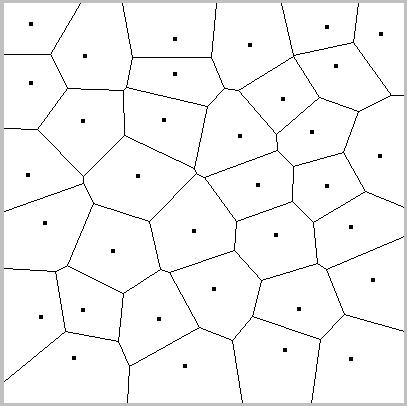
\includegraphics[width=4cm]{fig_6_1.jpg} 
	\caption{An example of Voronoi (or Dirichlet) tessellation, where we see a line connecting 2 points (centroids) will across orthogonally the boundary between the 2 points as implied by the nearest centroid rule.}\label{fig_6_1}
\end{figure}
\section{K-means}
\subsection{Basic Model}
K-means, as one of the most basic algorithm developed in 50s, formalizes the clustering problem as an optimization problem, where we aim to find centroids ${\bf u}_j\in\mathbb{R}^D$ and assignment $\pi$ that minimize a loss function or distortion, e.g. squared Euclidean norm. Concretely, we encode $\pi$ via an indicator matrix ${\bf Z}\in \{0,1\}^{N\times K}$, such that
\begin{equation*}
z_{ij}:=\begin{cases}
1&\text{if }\pi({\bf x}_i)=j\\
0&\text{otherwise}
\end{cases}.
\end{equation*}
Note that we have
\begin{equation*}
\sum_{j=1}^{K} z_{ij} = 1,\ \forall i.
\end{equation*}
The K-means objective function measures the distortion of replacing each data point by the assigned centroid and thus takes the form of
\begin{align}
\label{eq_6_km_obj}J({\bf U, Z})&=\sum_{i=1}^{N}\sum_{j=1}^{K} z_{ij}{\rm dist}({\bf x}_i, {\bf u}_j)=\sum_{i=1}^{N}\sum_{j=1}^{K} z_{ij}\|{\bf x}_i-{\bf u}_j\|^2\\
\label{eq_6_km_obj_mat}&=\|{\bf X-UZ}^T\|^2_F
\end{align}
where
\begin{align*}
&{\bf X} = [{\bf x}_1,\dots,{\bf x}_N]\in \mathbb{R}^{D\times N}\ \text{is the data matrix}\\
&{\bf U} = [{\bf u}_1,\dots,{\bf u}_K]\in \mathbb{R}^{D\times K}\ \text{is the centroid matrix.}
\end{align*}
We see that (\ref{eq_6_km_obj_mat}) is a matrix form of the original K-means objective function (\ref{eq_6_km_obj}) and is followed by
\begin{equation*}
(\ref{eq_6_km_obj}) = \sum_{i=1}^{N}\left\|{\bf x}_i-\sum_{j=1}^{K} z_{ij}{\bf u}_j\right\|^2 =  \sum_{i=1}^{N}\left\|{\bf x}_i-({\bf UZ}^T)_i\right\|^2 =(\ref{eq_6_km_obj_mat}).
\end{equation*}
The matrix form objective function (\ref{eq_6_km_obj_mat}) shows that K-means solves a matrix decomposition problem, where again we have a rank constraint that is introduced by $K$, and ${\bf Z}$ is not a real value matrix but a selection matrix with $z_{ij}\in\{0,1\}$.
\par As mentioned in section \ref{sec_4_EM}, directly minimizing the K-means objective (\ref{eq_6_km_obj}) is NP-hard, but we still have the following observations:
\begin{itemize}
	\item determining optimal centroids given assignments is easy (continuous variables)
	\item determining optimal assignments given centroids is easy (integer variables).
\end{itemize}
These two simple observations suggest an alternating minimization, i.e. the Lloyd's algorithm in section \ref{sec_4_EM}. Specifically, we alternatively
\begin{itemize}
	\item compute optimal assignment ${\bf Z}$, given centroids ${\bf U}$, by mapping each data point to the closest centroid since each data point contributes to exactly one term in the outer sum of objective (\ref{eq_6_km_obj})
	\begin{equation*}
	z_{ij}^*=\begin{cases}
	1&\text{if }j=\arg\min_k\|{\bf x}_i-{\bf u}_k\|^2\\
	0&\text{otherwise}
	\end{cases}
	\end{equation*}
	\item compute optimal choice of ${\bf U}$, given assignments ${\bf Z}$, by 1st order optimality condition, for non-empty clusters $(\sum_{i=1}^{N}z_{ij}\geq 1)$:
	\begin{equation*}
	\nabla_{{\bf u}_j}J({\bf U,Z})=\sum_{i=1}^{N}z_{ij}\nabla_{{\bf u}_j}\|{\bf x}_i-{\bf u}_j\|^2\overset{!}{=}0\Rightarrow {\bf u}_j^* =\frac{\sum_{i=1}^{N}z_{ij} {\bf x}_i}{\sum_{i=1}^{N}z_{ij}}
	\end{equation*}
	which is known as the centroid condition (center of mass of assigned data points).
\end{itemize}
We can initialize the centroids on $K$ distinct random data points (different initialization may be applied as well) and repeatedly do the above steps until the assignment does not change. With a consistent way to break the ties, where points have equal distances to multiple centroids, K-means algorithm will converge since the objective decrease monotonically, and the number of different assignment is large but finite. Note that the number of step of K-means algorithm until convergence can be very large for extreme cases. Since sometimes during the alternating optimization some clusters become empty, we can do random re-initialization to avoid this problem.
\begin{remark}
	The initialization of K-means can sometimes be problematic. Thinking about the example shown in Figure \ref{fig_6_2}, we see that with the illustrated initialization the final partition might have no cluster taking care of the points on the left. However, it is believed that with a "proper" initialization, K-means will perform well. We will also see more recent extensions of K-means that can handle these problematic cases in the following sections.
	\begin{figure}[h] 
		\centering 
		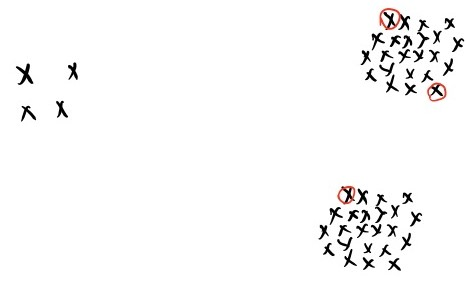
\includegraphics[width=5cm]{fig_6_2.jpg} 
		\caption{An example showing that sometimes the initialization will be problematic for K-means. Since there is no initial centroids in the left group, and there are far more points on the right, the final centroids will probably still be around the two groups to the right.}\label{fig_6_2}
	\end{figure}
\end{remark}
\par The computational cost of each iteration (2 steps) is $O(knd)$. Note that the number of step towards convergence can be very large, so the K-means algorithm can be quite expensive in the worst case. However, as mention before, K-means is guaranteed to converge. Although, the solution might not be global optimal since K-means optimizes a non-convex objective.
\begin{figure}[t] 
	\centering 
	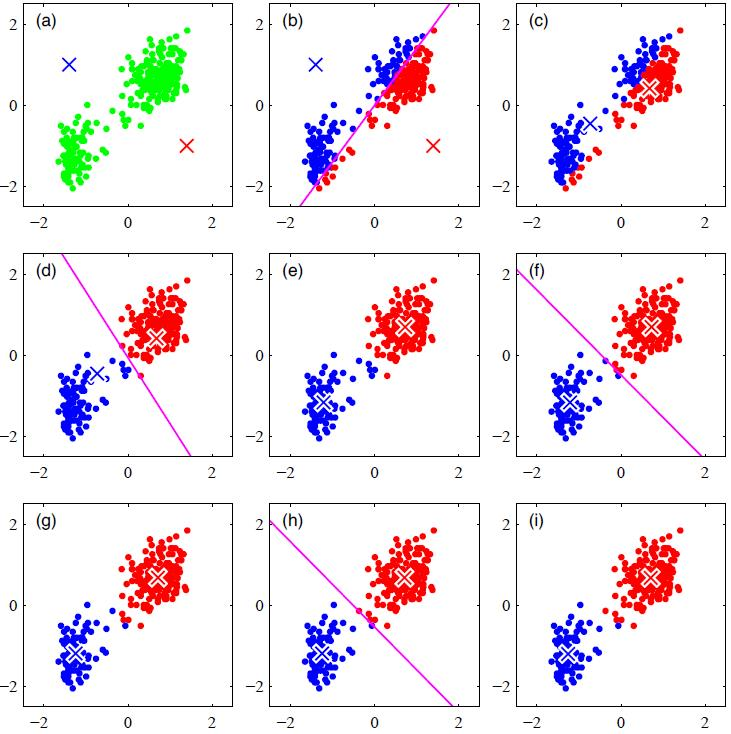
\includegraphics[width=7cm]{fig_6_3.jpg} 
	\caption{Illustration of the K-means algorithm. (Bishop 2006)}\label{fig_6_3}
\end{figure}
\subsection{K-mean++}
K-means++ suggests a more sophisticated seeding for initialization, which was introduced by Arthur \& Vassilvitskii, 2007 and has become a standard extension for K-means for really large data set. Recall that the failure case of random initialization for K-means shows that K-means may stuck at the beginning with at bad initialization. To remedy this, K-means++ suggests an \emph{incremental} $D^2$ (distance square) \emph{sampling} consisting of the following steps
\begin{itemize}
	\item Starting with an initial centroid set $\mathcal{U}_1=\{{\bf x}_I\}$, $I\sim {\rm Uniform}[1:N].$
	\item For $k=1,\dots,K-1$
	\begin{align*}
	&D_i:=\min_{{\bf u}\in \mathcal{U}_k}\|{\bf x}_i-{\bf u}\|,\quad \mathcal{U}_{k+1}:=\mathcal{U}_{k}\cup \{{\bf x}_i\},\ \text{where}\\
	&I\sim {\rm Categorical}({\bf p}),\quad p_i:=\frac{D_i^2}{\sum_{i=1}^{N}D_i^2}.
	\end{align*}
	Here in each step $k$, we construct a distribution according to the centroids that we have sampled, where points that are far from all sampled centroids will have large probabilities. Also, for the points that has been selected as a centroid it has $p_i=0$ since $D_i=0$, which makes sure that there will be no duplicated selection.
\end{itemize}
This sampling method is more expensive (can be implemented in a paralleled way for efficiency) than do thing all randomly, but gives consistently better experimental results. It has been proved that, K-means gives a theoretical guarantee: $O(\log K)$-competitiveness in expectation. Specifically, compared with the optimal clustering, K-means++ gives a solution that might be off by a $O(\log K)$ factor in terms of, say, sum of distortions in expectation. Although the $O(\log K)$ might not be so favorable, it avoids cases that K-means can be arbitrarily bad or fails completely.
\subsection{Core Set for K-means}
K-means++ provides a proper initialization, but K-means algorithm is still computationally expensive for very large data set. Imagine that we have 100 million users, and the question is do we really need so many data to identify groups? An intuitive idea is: maybe the analysis on properly-chosen 100 thousand users is enough to extrapolate the whole data set. However, can we do better to construct the subset than just do random sampling. This is exactly the question that the core set method for K-means aims to answer. The core set approach constructs a weighted sub-data-set on which we can run algorithms like K-means, and by construction we get guarantees of what holds for the large data set. This is a quite recent results by Bachem, Lucic, Krause, 2018: Scalable k-Means Clustering via Lightweight Coresets.
\par Mathematically speaking, K-means aims to find a set $\mathcal{U}$ of $k$ cluster centers in $\mathbb{R}^D$ such that the quantization error $\phi_{\mathcal{X}}(\mathcal{U})$ is minimize, where
\begin{equation}\label{eq_6_qe}
\phi_{\mathcal{X}}(\mathcal{U}) = \sum_{{\bf x}\in \mathcal{X}}{\rm d}({\bf x}, \mathcal{U})^2=\sum_{{\bf x} \in \mathcal{X}}\min_{{\bf u}\in \mathcal{U}} \|{\bf x-u}\|^2.
\end{equation}
For a weighted set $\mathcal{C}$ with corresponding weights ${\bf w}$, the quantization error is defined as
\begin{equation*}
\phi_{\mathcal{C}}(\mathcal{U}) = \sum_{{\bf x}\in \mathcal{C}}{\bf w}({\bf x}){\rm d}({\bf x},\mathcal{U})^2.
\end{equation*}
It is proved that, with the following way of sampling the core set, we have
\begin{equation}\label{eq_6_epsi_gua}
|\phi_{\mathcal{C}}(\mathcal{U}) - \phi_{\mathcal{X}}(\mathcal{U})|\leq \epsilon \phi_{\mathcal{X}}(\mathcal{U})
\end{equation}
with high probability for any $U \subset \mathbb{R}^D$. This shows that we have a control of the performance of K-means on the whole data set.
\par Concretely, we sample the core set, which can be a multi-set (with entries appears multiple times), of size $m$ in the following way. Note that different from K-means++, this is not initialization but sub-sampling data into a smaller set. We sample the core set from
\begin{equation*}
I\sim {\rm Categ}({\bf p}),\quad p_i:=\frac{1}{2N}+\frac{D_i^2}{2\sum_{j=1}^N D_j^2},\quad D_i^2=\|{\bf x}_i-\mu\|^2
\end{equation*}
where $\mu:=\frac{1}{N}\sum_i {\bf x}_i$ and each sample has a relative weight $\frac{1}{mp_i}$. The probability $p_i$ consists of 2 parts: the first component is the uniform distribution that ensures positivity; the second component is from the intuition that points which are far from the mean of the data have a potentially large impact on the quantization error (\ref{eq_6_qe}) of a clustering. The 2nd component ensures that these potentially important points are sampled frequently enough. As illustrated in Figure \ref{fig_6_4}, the proposed distribution makes points in the small group more likely to be selected.
\begin{figure}[t] 
	\centering 
	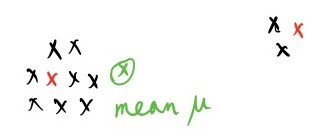
\includegraphics[width=5cm]{fig_6_4.jpg} 
	\caption{Illustration of the core set for K-means algorithm. All data points are represented as a cross with two red ones picked as members of the core set. The mean of the data is represented by the green cross in the circle. The way of sampling make sure that points that are far from the mean have greater probabilities, and the weights $\frac{1}{mp_i}$ compensate for low probabilities of important points near the mean.}\label{fig_6_4}
\end{figure}
\par To explain the role of the weights, we can again take a look at Figure \ref{fig_6_4}, where we have 2 points selected to form the core set. The points close to $\mu$ are with larger quantity but low probabilities, while points that are far from $\mu$ should be fewer but more likely to be chosen. As a result, we have one point from the larger group and one from the smaller cluster. Intuitively, if we want to recover the clustering property of the original data set, we should assign larger weights to the point that are close to $\mu$ to correct for the low probability in selection. The term $m$ in $\frac{1}{mp_i}$ is introduced to make the quantization error of the core set $\phi_{\mathcal{C}}(\mathcal{U})$ an unbiased estimator of the quantization error of the whole data set $\phi_{\mathcal{X}}(\mathcal{U})$. This can be justified by noting that
\begin{equation*}
\phi_{\mathcal{X}}(\mathcal{U}) = \sum_{{\bf x}\in \mathcal{X}}{\rm d}({\bf x}, \mathcal{U})^2 = \sum_{{\bf x}\in \mathcal{X}}p({\bf x})\frac{{\rm d}({\bf x}, \mathcal{U})^2}{p({\bf x})} = \mathbb{E}\left[\frac{{\rm d}({\bf x}, \mathcal{U})^2}{p({\bf x})}\right]
\end{equation*}
holds for any positive distribution $p({\bf x})$ over $\mathcal{X}$. The quantization error can hence be approximated by sampling $m$ points from $\mathcal{X}$ using $p({\bf x})$ and assigning them weights inversely proportional to $p({\bf x})$. Then we have an unbiased estimator (empirical expectation via sampling) of the $\phi_{\mathcal{X}}(\mathcal{U})$:
\begin{equation*}
\frac{1}{m}\sum_{{\bf x}\in \mathcal{C}}\frac{{\rm d}({\bf x},\mathcal{U})^2}{p({\bf x})} =\sum_{{\bf x}\in \mathcal{C}} \frac{1}{mp({\bf x})}{\rm d}({\bf x},\mathcal{U})^2 = \phi_{\mathcal{C}}(\mathcal{U}) \approx  \sum_{{\bf x}\in \mathcal{X}}p({\bf x})\frac{{\rm d}({\bf x}, \mathcal{U})^2}{p({\bf x})} =\phi_{\mathcal{X}}(\mathcal{U}).
\end{equation*}
It is proved that this approach gives $\epsilon$-approximation guarantees (\ref{eq_6_epsi_gua}) with probability at least $1-\delta$ for
\begin{equation*}
m\propto\frac{dk\log k+\log 1/\delta}{\epsilon^2}
\end{equation*}
which shows that the size of core set $\mathcal{C}$ is almost linear in $k$.
\begin{remark}
	Different from K-means++, in the core set sampling we have $D_i = \|{\bf x}_i-\mu\|$ which depends only on ${\bf x}_i$ and a fixed value $\mu=\frac{1}{N}\sum_i {\bf x}_i$. A natural question arises is that whether the distance to $\mu$ is enough to capture the structural properties of a specific point. The answer is probably that it is worth trying. However, we have to keep in mind that we almost always do not know the "right" thing to do, and the proposed core set method works out well for complete data as well in practice. This might suggest that it is better not to make assumptions that are too complicated.
\end{remark}
\section{Mixture Models}
This is a field in statistics that is closely related to K-means. One way to motivate the idea of mixture models is to go from hard assignments in K-means, where each data is assigned to exactly on cluster, to probabilistic assignments, where we want to assign ${\bf x}_i$ to each cluster $j$ with some probability $z_{ij}$. This leads to generalized or relaxed constraints on the selection matrix ${\bf Z}$ given by
\begin{equation*}
z_{ij}\in [0,1]\ (\forall i,j),\quad \sum_{j=1}^{K}z_{ij}=1\ (\forall i).
\end{equation*}
To do so, we can model each cluster by a probability distribution, which can be the multivariate normal distribution since it is the simplest choice. Just as a quick reminder, the PDF (probability density function) of univariate Gaussian with mean $\mu$ and variance $\sigma^2$ is defined as
\begin{equation*}
p(x;\mu,\sigma)=\frac{1}{\sigma\sqrt{2\pi}}\exp\left[-\frac{(x-\mu)^2}{2\sigma^2}\right],
\end{equation*}
and an isotropic multivariate normal distribution with mean $\bm{\mu}$ is given by
\begin{equation*}
p({\bf x};\bm{\mu},\sigma)=\prod_{i=1}^{D}\frac{1}{\sigma\sqrt{2\pi}}\exp\left[-\frac{(x_i-\mu_i)^2}{2\sigma^2}\right].
\end{equation*}
In a more general setting, a multivariate normal distribution with covariance matrix $\bm{\Sigma}$ takes the form of
\begin{equation*}
p({\bf x},\bm{\mu},{\bf \Sigma})=\frac{1}{|{\bf \Sigma}|^{\frac{1}{2}}(2\pi)^{\frac{D}{2}}}\exp\left[-\frac{1}{2 }({\bf x}-\bm{\mu})^T{\bf \Sigma}^{-1}({\bf x}-\bm{\mu})\right]
\end{equation*}
where ${\bf \Sigma}$ is symmetric and positive definite. Note that the setting with $\bm{\mu}$ and ${\bf \Sigma}$ is generally difficult to estimate for large $D$ since there are in total $D+\frac{D(D+1)}{2}$ parameters.
\par A finite mixture model is defined as a mixture of $k$ (simple) distribution with some mixing proportions
\begin{equation*}
p({\bf x};\theta)=\sum_{j=1}^{K}\pi_jp({\bf x};\theta_j),\quad \theta=(\pi,\theta_1,\dots,\theta_K)\in \mathbb{R}^{K+K\times M}
\end{equation*}
where $\theta$ are model parameters, and mixing proportions $\pi \geq 0,\ \sum_{j=1}^{K}\pi_j=1$. The density function of each component is given by $p({\bf x};\theta_j)$ with $\theta_j\in\mathbb{R}^M$. For mixture models for clustering, $\pi_j$ has an interpretation as the relative cluster size for cluster $j$ and serves as the probability for each cluster; the location and "shape" of cluster $j$ take a specific form of $p({\bf x};\theta_j)$. As a special case, for Gaussian mixture models, we have 
\begin{equation*}
\theta_j=(\underbrace{\bm{\mu}_j}_{\rm location},\underbrace{{\bf \Sigma_j}}_{\rm shape}).
\end{equation*}
A Gaussian mixture model (GMM) hence takes the form of
\begin{equation*}
p({\bf x};\theta)=\sum_{j=1}^{K}\pi_j p({\bf x};\bm{\mu}_j,{\bf \Sigma}_j).
\end{equation*}
This suggests a two-stage generative model: we can generate a data point as follows
\begin{enumerate}
	\item sample cluster index from categorical distribution $j\sim {\rm Categorical}(\pi)$
	\item given $j$, sample a data point ${\bf x}$ from the $j^{\rm th}$ component $\mathcal{N}(\bm{\mu}_j,{\bf \Sigma}_j)$.
\end{enumerate}
Here cluster index $j$ is a latent variable, and the final outcome ${\bf x}$ is what we actually observed. Mathematically speaking, the goal of probabilistic clustering is to compute posteriors of latent cluster memberships. The following part is discussed in more details in section \ref{sec_4_EM}, for maintaining the complete structure of the notes we will briefly discuss it again here.
\par By explicitly introducing latent variables into generative models, hopefully we can simplify the calculations. Concretely, we attach a assignment variable ${\bf z}$ to each data point ${\bf x}$ to form a generic (or complete) data point $({\bf x,z})$, where
\begin{equation*}
{\bf z}\in\{0,1\}^{K},\quad \sum_{j=1}^{K}z_j=1.
\end{equation*}
The latent variable ${\bf z}$ obeys a categorical distribution
\begin{equation*}
\mathcal{P}(z_j=1)=\pi_j\quad {\rm or}\quad p_{\pi}({\bf z}) =\prod_{j=1}^{K}\pi_j^{z_j}.
\end{equation*}
Thus, the joint distribution over $({\bf x, z})$ (\textbf{complete data} distribution) is given by
\begin{equation*}
p({\bf x,z};\theta) = p({\bf z};\theta)p({\bf x}|{\bf z};\theta) = \prod_{j=1}^{K}\pi_j^{z_j} \prod_{j=1}^{K}p({\bf x};\theta_j)^{z_j} = \prod_{j=1}^{K}[\pi_jp({\bf x};\theta_j)]^{z_j}
\end{equation*}
where we have used that $p({\bf x}|{\bf z};\theta) =\prod_{j=1}^{K}p({\bf x};\theta_j)^{z_j}$. With these probabilities, we can play with the posterior assignments. Note that probabilistically speaking, \emph{data generation} is to generate data points ${\bf x}$ given cluster assignments ${\bf z}$, and data inference is to infer cluster assignment ${\bf z}$ given a specific data point ${\bf x}$. Recall that we can compute the posterior by the Bayes rule
\begin{equation*}
{\rm posterior}\ p(A|B)=\frac{p(B|A)p(A)}{p(B)}
\end{equation*}
where $p(A)$ is the prior, $p(B|A)$ is the likelihood, and $p(B)$ refers to evidence. The posterior probabilities for assignments is therefore
\begin{equation*}
\mathbb{P}(z_j=1|{\bf x})=\frac{\mathbb{P}(z_j=1)p({\bf x}|z_j=1)}{\sum_{l=1}^{K}\mathbb{P}(z_l=1)p({\bf x}|z_l=1)}=\frac{\pi_jp({\bf x};\theta_j)}{\sum_{l=1}^{K}\pi_lp({\bf x};\theta_l)}
\end{equation*}
where we have assumed access to parameters $\pi, \{\theta_j=(\bm{\mu}_j,{\bf \Sigma}_j)\}$. Suppose that all the data points are drawn independently. The maximum likelihood estimation (MLE) of mixture models requires to optimize
\begin{equation}\label{eq_6_mixture_mle}
\hat{\theta} = \mathop{\arg\max}_{\theta} \sum_{i=1}^{N}\log p({\bf x}_i;\theta) = \mathop{\arg\max}_{\theta} \sum_{i=1}^{N}\log \left[\sum_{j=1}^{K} \pi_jp({\bf x}_i;\theta_j)\right].
\end{equation}
However, the summation over $j$ inside the logarithm prevents a analytical closed-form solution. A remedy to this problem is the Expectation Maximization (EM) algorithm, which maximize a lower bound on the log-likelihood based on complete data distribution. Specifically
\begin{align}
\log p({\bf x;\theta})&=\log \left[\sum_{j=1}^{K} \pi_jp({\bf x};\theta_j)\right]=\log \left[\sum_{j=1}^{K} q_j \frac{\pi_jp({\bf x};\theta_j)}{q_j} \right]\notag\\
\label{eq_6_em_bd}&\geq \sum_{j=1}^{K}q_j[\log p({\bf x};\theta_j) +\log \pi_j - \log q_j]
\end{align}
where $q_j$ is a distribution over $j=1,\dots,K$, such that $q_j>0,\ \sum_j q_j=1$, and the inequality follows by the Jensen's inequality noting the concavity of logarithm. Note that the summation over $i$ in MLE objective (\ref{eq_6_mixture_mle}) is outside of the logarithm, so we can evaluate the contribution of each data point ${\bf x}_i$ by the proposed lower bound separately (additive).
\par In the expectation step (E-step), we optimized bound (\ref{eq_6_em_bd}) with regard to the distribution $q$. We formulate the following Lagrangian (decoupled for each data point)
\begin{equation*}
\max_{q}\left\{\sum_{j=1}^{K}q_j[\log p({\bf x};\theta_j) +\log \pi_j - \log q_j] +\lambda (\sum_{j=1}^{K}q_j -1) \right\}.
\end{equation*}
Apply the first order optimality condition (setting gradient to zero) we get:
\begin{align*}
&\log p({\bf x};\theta_j) +\log \pi_j - \log q_j - 1 +\lambda \overset{!}{=}0 \Longleftrightarrow\\
&q_j^*=\frac{\pi_jp({\bf x};\theta_j)}{\sum_{l=1}^{K}\pi_lp({\bf x};\theta_l)}\overset{\rm Bayes\ rule}{=}\mathbb{P}(z_j=1|{\bf x})
\end{align*} 
which shows that the optimal $q$-distribution equals to the posterior given the parameters. In another word, E-step selects the best lower bound on the log-likelihood given ${\bf \theta}$.
\par In the maximization step (M-step), we optimize expected complete data log-likelihood with regard to the model parameters. Note that the problem decouples for each cluster and with regard to $\pi$. Specifically, combining the MLE objective (\ref{eq_6_mixture_mle}) and the lower bound for each point (\ref{eq_6_em_bd}), we get
\begin{align}
\label{eq_6_em_bd_cplt}\sum_{i=1}^{N}\log p({\bf x}_i;\theta) &\geq \sum_{i=1}^{N}\sum_{j=1}^{K}q_{ij}[\log p({\bf x}_i;\theta_j) +\log \pi_j - \log q_{ij}]\\
&=\sum_{i=1}^{N}\sum_{j=1}^{K}q_{ij}\log p({\bf x}_i|z_{ij}=1;\theta)p(z_j=1) -q_{ij}\log q_{ij}\notag\\
\label{eq_6_em_bd_ana}&=\sum_{i=1}^{N}\sum_{j=1}^{K}\mathbb{P}(z_j=1|{\bf x}_i)\log p({\bf x}_i,z_j=1;\theta) +{\rm const}
\end{align}
where $q_{ij}$ and $z_{ij}$ are the $q_j$ in (\ref{eq_6_em_bd}) and $z_j$ for ${\bf x}_i$ respectively, and we have assumed fixed $q_{ij} = \mathbb{P}(z_j=1|{\bf x}_i)$; the constant is for that they are only related to $q_{ij}$. If we write the first term of (\ref{eq_6_em_bd_ana}) in a matrix form, we get
\begin{equation*}
\sum_{\bf Z}\mathbb{P}({\bf Z}|{\bf X})\log p({\bf X,Z};\theta)=\mathbb{E}_{\bf Z|X}\log p({\bf X,Z};\theta)
\end{equation*}
which shows that we are optimizing the expected complete data log-likelihood. Given fixed $q_{ij} = \mathbb{P}(z_j=1|{\bf x}_i)$, we can again apply the first order optimality condition with Lagrangian to solve for optimal $\pi$ and $ \theta_j = (\bm{\mu}_j,\bm{\Sigma}_j)$:
\begin{align*}
&\nabla_{\pi_j}\left[\sum_{i=1}^{N}\sum_{j=1}^{K}q_{ij}\log \pi_j +\lambda(\sum_{l=1}^{K} \pi_l-1)\right]\overset{!}{=}0\Rightarrow \pi_j^* =\frac{1}{N}\sum_{i=1}^{N}q_{ij}\\
&\nabla_{\bm{\mu}_j}\sum_{i=1}^{N}\sum_{j=1}^{K}q_{ij}\log \mathcal{N}({\bf x}_i;\bm{\mu}_j,{\bf \Sigma}_j) \overset{!}{=}0\Rightarrow \bm{\mu}_j^*=\frac{\sum_{i=1}^{N}q_{ij}{\bf x}_i}{\sum_{i=1}^{N}q_{ij}}\\
&\nabla_{\bm{\Sigma}_j}\sum_{i=1}^{N}\sum_{j=1}^{K}q_{ij}\log \mathcal{N}({\bf x}_i;\bm{\mu}_j,{\bf \Sigma}_j) \overset{!}{=}0\Rightarrow \bm{\Sigma}_j^*=\frac{\sum_{i=1}^{N}q_{ij}({\bf x}_i-\bm{\mu}_j)({\bf x}_i-\bm{\mu}_j)^T}{\sum_{i=1}^{N}q_{ij}}.
\end{align*}
Solving the optimal covariance matrix needs some extra tool of matrix derivative, where one might need:
\begin{equation*}
\frac{\partial}{\partial {\bf A}}\ln |{\bf A}|=({\bf A}^{-1})^T,\ \frac{\partial}{\partial {\bf A}} {\rm Tr}({\bf AB})={\bf B}^T.
\end{equation*}
The EM algorithm works by alternate E-steps and M-steps, and both E and M step are maximizing the same objective. As in K-means, it is guaranteed to converge towards a point $\theta^*$ (with some convergence criteria), while, again like in K-means, $\theta^*$ may not be the global maximizer. As a summary, we have
\begin{itemize}
	\item E-step: compute probabilistic assignments of points to clusters (keeping their location and shape fixed)
	\item M-step: recompute optimal cluster locations and shapes, given probabilistic assignments.
\end{itemize}
\begin{figure}[h] 
	\centering 
	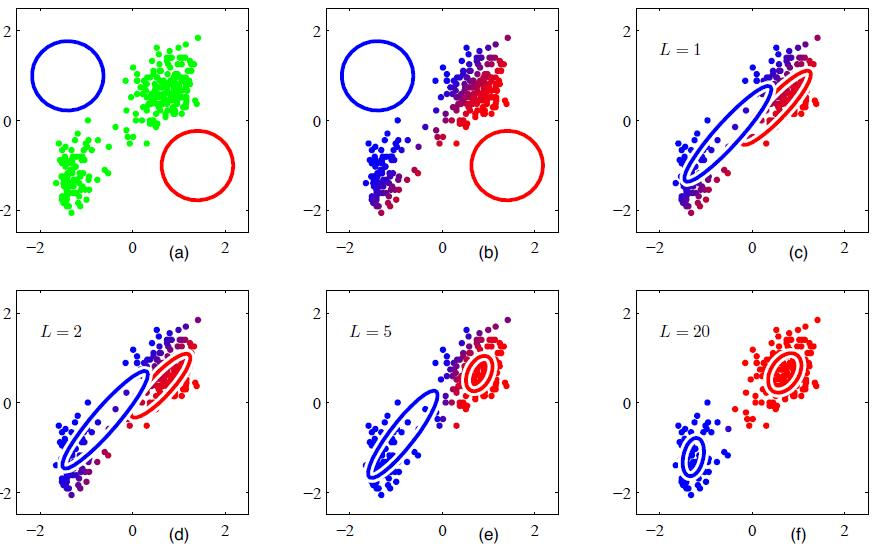
\includegraphics[width=10cm]{fig_6_5.jpg} 
	\caption{Gaussian mixture model fitting via EM for two clusters. Remark: here the covariance is also estimated (illustrated by the two ellipsoids). (Bishop 2006)}\label{fig_6_5}
\end{figure}
To conclude this section, we now spend some time comparing the two clustering algorithms mentioned up to now:
\begin{itemize}
	\item Assignments:
	\begin{itemize}
		\item K-means algorithm: hard assignment points to clusters
		\item EM algorithm: soft assignment based on posteriors
	\end{itemize}
	\item Shapes:
	\begin{itemize}
		\item K-means: spherical cluster shapes, uniform spread
		\item EM: can learn covariance matrix (ellipsoid-shaped)
	\end{itemize}
	\item K-means as a special case: as discussed in section \ref{sec_4_em_km_compare}, K-means can be regarded as a special case of Gaussian mixture models with (fixed) covariance ${\bf \Sigma}_j=\sigma^2{\bf I}$ in the limit of $\sigma \rightarrow 0$ (hard assignment).
\end{itemize}
\par In practice, EM algorithm takes much more iterations to converge and in each cycle requires significantly more computation. In this case, K-means can be used to find a good initialization of the EM: covariance matrices can be initialized to the sample covariances of the clusters found by the K-means algorithm; mixing coefficients can be set to the fractions of data points assigned to the respective clusters.
\section{Model Selection}
The last topic of this chapter is about model selection which is often motivated by this kind of questions: what is the proper number of model parameters, or how should we determine the model complexity? In a typical machine learning task people usually have to find trade-off between two conflicting goals:
\begin{itemize}
	\item Data fit: We want to predict the data well, e.g., maximizing the data log-likelihood. In this case, usually more complex model gives better fit on the observed data.
	\item Complexity: Choose a model that is not very complex which is often measured by the number of free parameters. Too complex models tend to over fit the observed data and give bad generalization power.
\end{itemize}
Take the number of clusters in a data clustering problem as an example. Recall that the negative log-likelihood of data for $K$ mixture Gaussians can be written as
\begin{equation*}
-\log p({\bf X};\theta)=-\sum_{i=1}^{N}\log \left[\sum_{j=1}^{K}\pi_jp({\bf x}_i;\theta_j)\right].
\end{equation*}
For one specific clustering algorithm like K-means, the negative log-likelihood v.s. number of clusters $K$ usually takes the form as illustrated in Figure \ref{fig_6_6}. Note that smaller negative log-likelihood means better fit (to the observed data). As illustrated, in general the objective decreases with $K$ (some noise due to local minima), but very small does not necessarily mean a good fit. 
\begin{figure}[h] 
	\centering 
	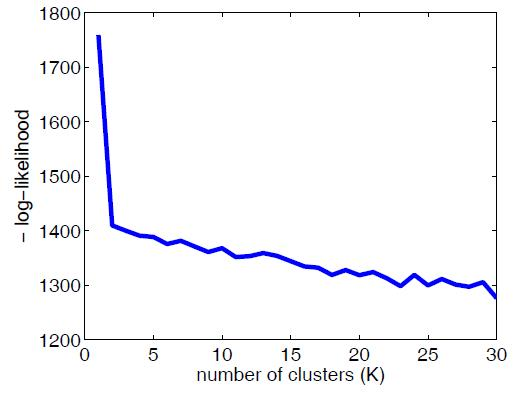
\includegraphics[width=5cm]{fig_6_6.jpg} 
	\caption{A typical negative log-likelihood plot of clustering algorithms}\label{fig_6_6}
\end{figure}
\par If we measure the model complexity by the number of free parameters $\kappa(\cdot)$, there are two heuristics for choosing $K$:
\begin{itemize}
	\item Akaike Information Criterion (AIC):
	\begin{equation*}
	{\rm AIC}(\theta|{\bf X})=-\log p({\bf X};\theta)+\kappa(\theta)
	\end{equation*}
	\item Bayesian information Criterion (BIC):
	\begin{equation*}
	{\rm BIC}(\theta|{\bf X})=-\log p({\bf X};\theta)+\frac{1}{2}\kappa(\theta)\log N
	\end{equation*}
\end{itemize}
Generally speaking, the BIC criterion penalizes complexity more than the AIC criterion. Note that a single AIC (BIC) result is meaningless. One has to repeat the analysis for different $K$ and compare the differences: the most suitable number of clusters corresponds to the smallest AIC (BIC) value. As an example, we can consider a mixture of Gaussians:
\begin{itemize}
	\item Number of free parameters (with fixed covariance matrices) is
	\begin{equation*}
	\kappa(\theta)=\underbrace{K\cdot D}_{\bm{\mu}}+\underbrace{(K-1)}_{\pi}
	\end{equation*}
	\item Number of free parameters (with full covariance matrices) is given by
	\begin{equation*}
	\kappa(\theta)=K\cdot\left(\underbrace{D}_{\bm{\mu}} +\underbrace{\frac{D(D+1)}{2}}_{\bm{\Sigma}} \right)+\underbrace{(K-1)}_{\pi}.
	\end{equation*}
\end{itemize}
Figure \ref{fig_6_7} and Figure \ref{fig_6_8} illustrate AIC and BIC examples for 3 and 5 clusters respectively. We can see that in both case, the minimal values of BIC and AIC value correspond to the "right" number of clusters.
\begin{figure}[h] 
	\centering 
	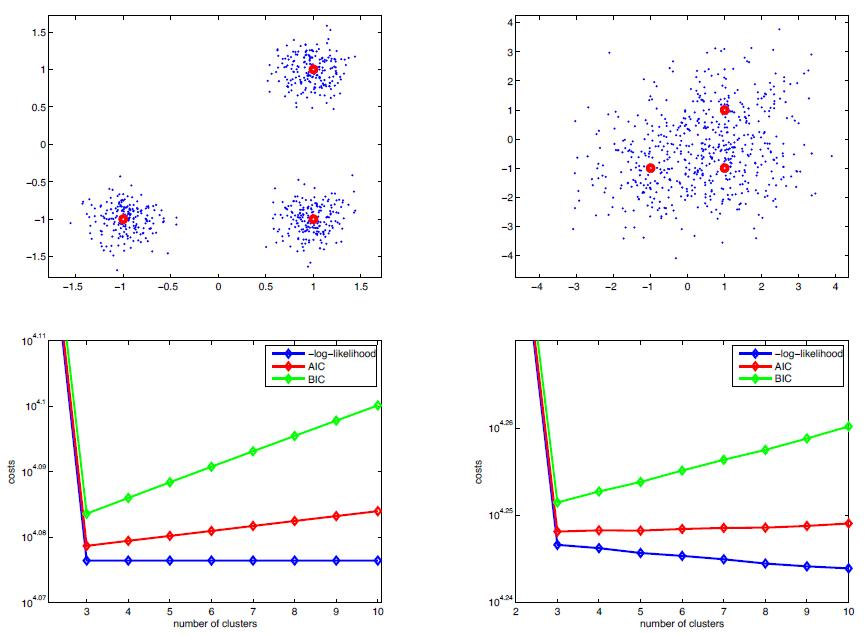
\includegraphics[width=12cm]{fig_6_7.jpg} 
	\caption{Information criteria for a synthetic dataset with 3 clusters. Synthetic data has smaller variance on the left than on the right.}\label{fig_6_7}
\end{figure}
\begin{figure}[h] 
	\centering 
	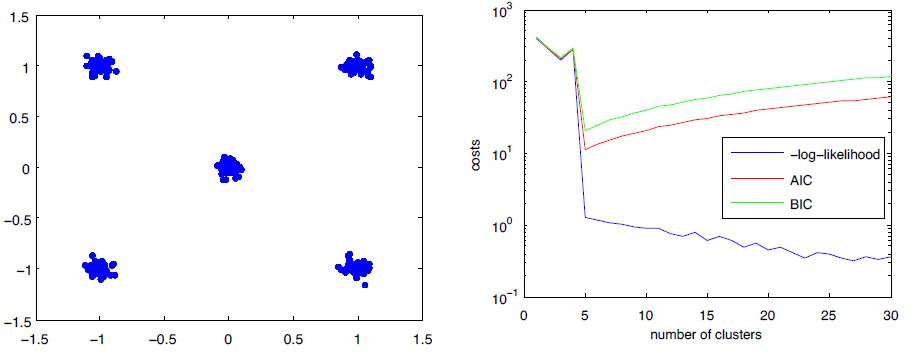
\includegraphics[width=12cm]{fig_6_8.jpg} 
	\caption{Information criteria for a synthetic dataset with 5 clusters.}\label{fig_6_8}
\end{figure}
\end{document}